\documentclass{standalone}
\usepackage{tikz}

\begin{document}
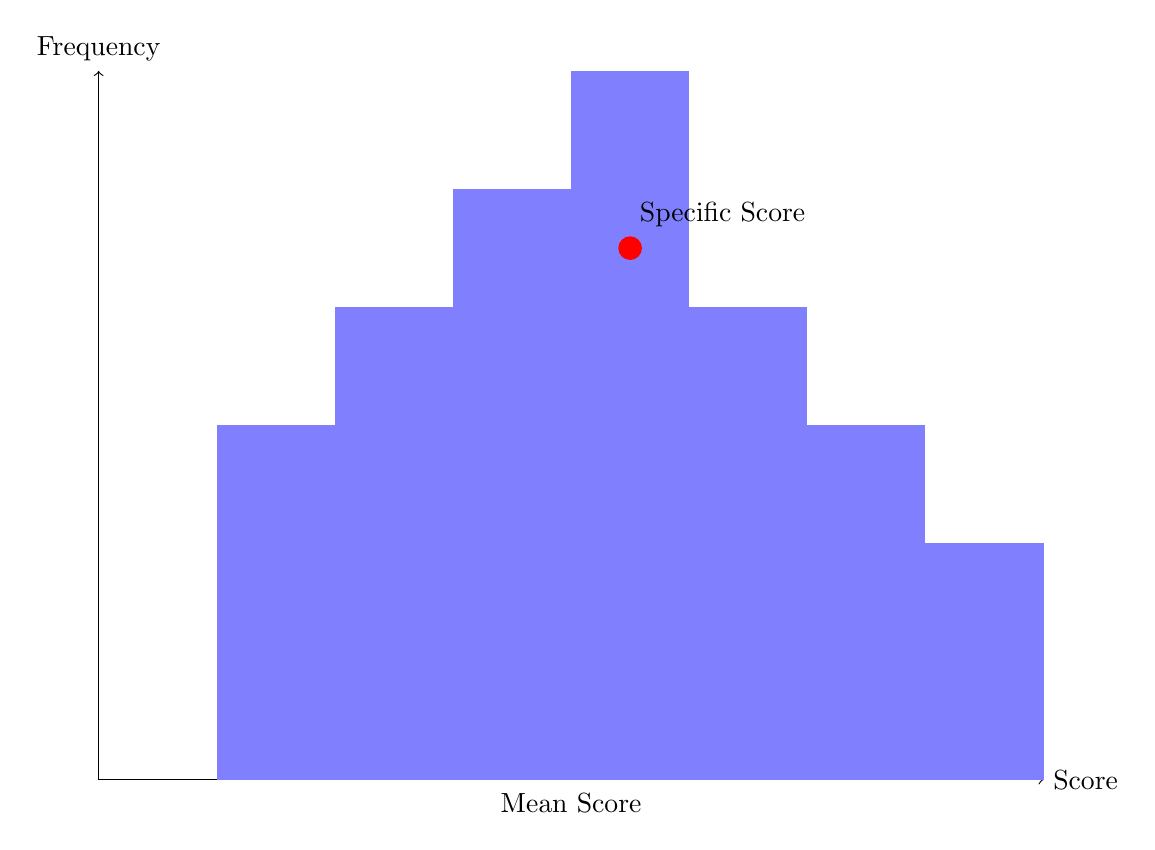
\begin{tikzpicture}[scale=1.5]
    % Set up the axes
    \draw[->] (0,0) -- (8,0) node[right] {Score};
    \draw[->] (0,0) -- (0,6) node[above] {Frequency};

    % Draw the histogram bars
    \fill[blue!50!white] (1,0) rectangle (2,3);
    \fill[blue!50!white] (2,0) rectangle (3,4);
    \fill[blue!50!white] (3,0) rectangle (4,5);
    \fill[blue!50!white] (4,0) rectangle (5,6);
    \fill[blue!50!white] (5,0) rectangle (6,4);
    \fill[blue!50!white] (6,0) rectangle (7,3);
    \fill[blue!50!white] (7,0) rectangle (8,2);

    % Add a red dot at a specific score
    \fill[red] (4.5,4.5) circle[radius=0.1];

    % Add labels
    \node at (4,-0.2) {Mean Score};
    \node at (4.5,4.6) [anchor=south west] {Specific Score};
\end{tikzpicture}
\end{document}